\chapter{Theory and motivation}
\label{sec:theory}

The \ac{SM} of particle physics is our current best theory to describe the fundamental particles and their interactions.
The \ac{SM} describes the strong force, as well as unifying the weak and electromagnetic forces.
The latter is partly done through the \ac{BEH} mechanism for spontaneous symmetry breaking, that allows many fundamental particles to obtain masses.
It also predicts a new scalar boson, named the Higgs boson.
In 2012, the ATLAS~\cite{ATLAS_Higgs_Discovery} and CMS~\cite{CMS_Higgs_Discovery} collaborations discovered a Higgs boson-like particle when colliding protons at high energies at the \ac{LHC}. 
Further measurements of the particle's properties have been consistent with the \ac{SM} prediction.
This discovery experimentally completed the \ac{SM} particle constituents. \\

However, the \ac{SM} is not without theoretical problems and experimental tensions.
Firstly, the hierarchy problem describes the issue of lightness of the observed Higgs boson mass and the \say{unnatural} balancing of inputs needed to explain the theorised loop corrections to the predicted mass. 
These are orders of magnitude larger than the observed mass.
A solution to this problem is \ac{SUSY}, but no experimental evidence for this theory has yet been found that separates it from the \ac{SM}. 
Secondly, results from B physics~\cite{LHCb:2021trn,Kowalewski:2013mna,BaBar:2013mob,Belle:2015qfa,LHCb:2015gmp,Belle:2016dyj,LHCb:2017rln,LHCb:2017smo} and the measurement of the muon's anomalous magnetic moment~\cite{Muong-2:2006rrc,Muong-2:2021ojo} have shown deviations from the \ac{SM} predictions.
Although not the statistical significance for a discovery, they offer intriguing hints at potential \ac{BSM} physics.
\ac{BSM} particles, produced from extended Higgs sectors or otherwise, have been theorised to explain these deviations.
This chapter will explain the \ac{SM} and the Higgs sector theory, as well as detailing the \ac{BSM} extensions that can help resolve the theoretical problems and experimental tensions. \\

One caveat to the B physics results presented in this thesis, is the exclusion of the updated $\text{R}_{\text{K}}$ and $\text{R}_{\text{K}^{*}}$ measurements from the LHCb collaboration~\cite{LHCb:2022zom}.
This is due to the interpretation of the B anomalies, described in this chapter and used in Chapter~\ref{sec:bsm_H_to_tau_tau_analysis}, being concluded prior to the release of Reference~\cite{LHCb:2022zom}.
The phenomenological effect of Reference~\cite{LHCb:2022zom}, on the best fit of new physics to the B anomalies, is yet to be fully determined.

\section{The Standard Model of particle physics}

\subsection{Fundamental particles and their interactions}

The \ac{SM} is a set of fundamental particles, as shown in Figure~\ref{fig:sm_diagram}, and rules that govern the interactions between particles.
The interactions between these particles are able to model the strong, weak and electromagnetic force, unifying the later two into one electroweak interaction.
The \ac{SM} consists of 6 quarks, 3 charged leptons and 3 neutrinos, which are grouped into \say{fermions} because of their shared half integer spin. 
Each of these particles has an anti-partner with opposite quantum numbers but the same mass.
The \ac{SM} also consists of a number of particles, named \say{bosons}, with shared integer spin, that describe the fundamental forces of nature: the strong, weak, and electromagnetic forces. 
The gluon is the mediator of the strong force, the W and Z bosons mediate the weak force, and the photon mediates the electromagnetic force. \\

\begin{figure}[!hbtp]
\centering
    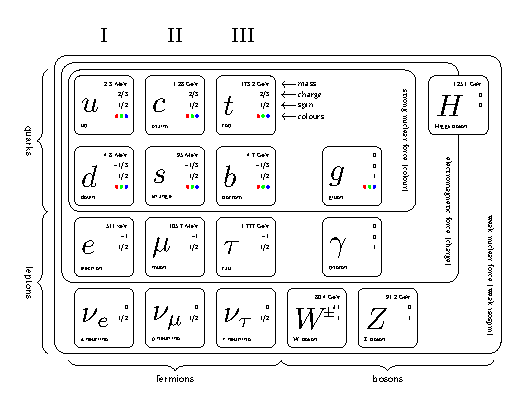
\includegraphics[width=0.99\textwidth]{Figures/SM_diagram.pdf}
\caption{Diagram of the fundamental particles that constitute the SM. Also displayed are the fermion generation shown in Roman numerals, the particles measured mass, charge, spin and colours available for the strong interaction. This particle masses used are from Reference~\cite{ParticleDataGroup:2022pth}. The neutrino masses are left blank as the values are unknown. This figure is taken and adjusted from Reference~\cite{sm_diagram}.}
\label{fig:sm_diagram}
\end{figure}

The \ac{SM} is a renormalisable quantum field theory that is built on the principle of local gauge invariance.
The SU(3)$_{\text{C}}$ $\otimes$ SU(2)$_{\text{L}}$ $\otimes$ U(1)$_{\text{Y}}$ is the gauge symmetry group of the \ac{SM}.
This means that the Lagrangian, that governs the particles interactions, is invariant under such a transformation. 
SU(2)$_{\text{L}}$ $\otimes$ U(1)$_{\text{Y}}$ is the symmetry of the electroweak unification and SU(3)$_{\text{C}}$ is the symmetry of the theory for strong force, name \ac{QCD}. \\

The quantum number associated with the \ac{QCD} SU(3)$_\text{C}$ symmetry is the colour charge C.
Quarks and gluons carry a colour charge and so interact with the strong force.
One characteristic feature of \ac{QCD} is confinement, which requires neutral colour charges and so quarks must be observed in a bound state, named hadrons.
Another key property is asymptotic freedom, which weakens the interaction strength at higher energy or very short distances \cite{Gross:1973id,Politzer:1973fx}. \\

Electroweak unification was initially proposed by Glashow~\cite{Glashow:1961tr}, Weinberg~\cite{Weinberg:1967tq} and Salam~\cite{Salam:1968rm} to combine the theories for the weak and electromagnetic forces into one.
It is built on the premise of the Dirac equation.
The Dirac Lagrangian for a massless spinor field, $\psi$, is defined as,

\begin{equation}
\mathcal{L}_{\text{Dirac}} = i\bar{\psi}\gamma^{\mu} \partial_{\mu} \psi,
\end{equation}

where $\gamma^{\mu}$ are the gamma matrices and $\partial_{\mu}$ are partial derivatives.
The SU(2)$_{\text{L}}$ transformation operates on the weak isospin, $I$, only for the left-handed spinors and the U(1)$_{\text{Y}}$ transformation operates on the weak hypercharge, $Y=2(Q-I_{3})$, where Q is the charge of the fundamental particles and $I_3$ is the third component of the weak ispospin.
The reason for the distinction of the SU(2) symmetry to act only on left-handed spinors is from the observed chirality of fermions under the weak interaction.
By invoking gauge invariance of the Dirac Lagrangian under such a transformation, four associated gauge fields are present, $\boldsymbol{W}_{\mu} = (W^{1}_{\mu},W^{2}_{\mu},W^{3}_{\mu})$ and $B_{\mu}$.
The Lagrangian then takes the form,

\begin{align}
\begin{split}
\mathcal{L}_{\text{Electroweak}} &= \bar{\psi}_{L}\Big(\partial_{\mu} + \frac{i}{2} g \boldsymbol{W}_{\mu} \cdot \boldsymbol{\sigma} + g^{\prime} Y B_{\mu}  \Big) \psi_L \\
&+ \bar{\psi}_{R}\Big(\partial_{\mu} + + g^{\prime} Y B_{\mu}  \Big) \psi_R - \frac{1}{4} \boldsymbol{W}_{\mu\nu} \cdot \boldsymbol{W}^{\mu\nu} - \frac{1}{4}B_{\mu\nu}B^{\mu\nu},
\end{split}
\end{align}

where $g$ and $g^{\prime}$ are the coupling constants for the SU(2) and U(1) symmetries respectively, the partial derivatives have been replaced with the covariant derivative and the added field tensors $\boldsymbol{W}_{\mu\nu}$ and $B_{\mu\nu}$ are defined as,

\begin{equation}
\boldsymbol{W}_{\mu\nu} = \partial_{\mu} \boldsymbol{W}_{\nu} - \partial_{\nu} \boldsymbol{W}_{\mu} - ig[\boldsymbol{W}_{\mu},\boldsymbol{W}_{\nu}],
\end{equation}

\begin{equation}
B_{\mu\nu} = \partial_{\mu} B_{\nu} - \partial_{\mu} B_{\mu}.
\end{equation}

These fields can be rotated into the physical fields for the photon, Z and W boson with the following transformations,

\begin{align}
\begin{split}
W^{\pm}_{\mu} &= \frac{1}{\sqrt{2}}(W^{1}_{\mu} \mp W^{2}_{\mu}), \\
Z_{\mu} &= W^{3}_{\mu} \cos\theta_{w} - B_{\mu} \sin\theta_w, \\
A_{\mu} &= W^{3}_{\mu} \sin\theta_{w} - B_{\mu} \cos\theta_w,
\end{split}
\label{eqn:rotations}
\end{align}

where $\theta_w$ represents the weak mixing angle and is defined such that

\begin{equation}
\sin\theta_w = \frac{g^{\prime}}{\sqrt{g^2 + g^{\prime 2}}}, \hspace{1cm} \cos\theta_w = \frac{g}{\sqrt{g^2 + g^{\prime 2}}}.
\end{equation}

The W and Z bosons were discovered by the UA1 and UA2 collaborations in 1983 \cite{UA1:1983crd,UA2:1983tsx}, which confirmed the predictions made by electroweak unification.
However, the W and Z bosons were measured to have a non-zero mass and Lagrangian mass terms of the form $\frac{1}{2}m_{Z}^2 Z_{\mu} Z^{\mu}$ or $m_{W}^2 W_{\mu}^{-}W^{+\mu}$ cannot be included as they are not invariant under the SU(2)$_{\text{L}}$ $\otimes$ U(1)$_{\text{Y}}$ gauge symmetry.
The same issue also exists in massive fermions, as the fermion mass term's left- and right-handed chiral states, $m\bar{\psi}\psi = m(\bar{\psi}_R \psi_L + \bar{\psi}_L \psi_R)$,  transform differently and therefore does not remain invariant under the gauge transformation.
To resolve this, the \ac{BEH} mechanism for spontaneous symmetry breaking was theorised.

\subsection{Higgs sector}

The \ac{BEH} mechanism was proposed in the 1960s by Englert and Brout~\cite{Englert:1964et}, Higgs~\cite{Higgs:1964ia,Higgs:1964pj,Higgs:1966ev} and Guralnik, Hagen and Kibble~\cite{Guralnik:1964eu,Kibble:1967sv}.
It works on the principles of spontaneous symmetry breaking of the SU(2)$_{\text{L}}$ $\otimes$ U(1)$_{\text{Y}}$ gauge symmetry.
It does this by introducing a gauge invariant field that has a non-zero \ac{VEV}.
The formalism of this is shown below, starting from a complex scalar doublet, $\Phi$. 

\begin{equation}
	\Phi = 
	\begin{pmatrix} 
		\phi^{+} \\
		\phi^{0} \\
	\end{pmatrix},
\end{equation}

where $\phi^{+}$ and $\phi^{0}$ are complex functions.
The Lagrangian and the potential, chosen to fulfil the conditions stated above, then takes the form,

\begin{equation}
	\mathcal{L}_{\text{Complex Scalar}} = (\partial_{\mu}\Phi)^{\dagger} (\partial^{\mu}\Phi) - V(\Phi),
\end{equation}

with,

\begin{equation}
V(\phi) = \mu^2 \Phi^{\dagger} \Phi + \lambda (\Phi^{\dagger} \Phi)^2,
\end{equation}

where $\mu^2$ and $\lambda$ are two real parameters. 
$\lambda$ is required to be positive for the vacuum to be stable.
If $\mu^2$ is negative, $\Phi$ will have a non-zero \ac{VEV} and the field will be able to spontaneously break the gauge symmetry.
In the vacuum state, the field must satisfy the criteria,

\begin{equation}
\Phi^{\dagger} \Phi = -\frac{\mu^2}{2\lambda}.
\end{equation}

This potential fulfils the criteria of a non-zero \ac{VEV} as $\Phi$ must be non-zero. 
Choosing a gauge to remove the massless scalar bosons, predicted by Goldstone's theorem~\cite{Goldstone:1961eq}, by taking $\phi^+$ to be zero and $\phi$ to be real.
The ground state of $\Phi$ is found as,

\begin{equation}
\braket{0|\Phi|0} = \frac{1}{\sqrt{2}}
	\begin{pmatrix} 
		0 \\
		\nu \\
	\end{pmatrix},
\end{equation}

where $\nu^2 = \mu^2 / \lambda$ and $\nu$ is the non-zero \ac{VEV}.
The complex doublet can then be written as an expansion around the minimum of the potential,

\begin{equation}
\Phi = \frac{1}{\sqrt{2}}
	\begin{pmatrix} 
		0 \\
		\nu + h(x)\\
	\end{pmatrix}
\end{equation}

Applying the covariant derivative for the electroweak gauge symmetry to produce the Lagrangian for the field, $\Phi$, yields

\begin{align}
\begin{split}
\mathcal{L}_{\text{Higgs}} &= \frac{1}{2}(\partial_{\mu}h)(\partial^{\mu}h) + \frac{1}{8} g^{2} (W_{\mu}^{1} + i W_{\mu}^{2})(W^{1\mu} - i W^{2\mu})(\nu + h)^2 \\
&+ \frac{1}{8} (g W_{\mu}^{3} - g' B_{\mu})(g W^{3\mu} - g' B^{\mu})(\nu + h)^2  \\
&+ \mu^2 (\nu + \Ph)^2 + \lambda (\nu + h)^4.
\end{split}
\end{align}

Mass terms for $W_{\mu}^{1}$ and $W_{\mu}^{2}$ are now present and hence the mass of the W boson is $m_W = \frac{1}{2}g\nu$.
Once again, the remaining states need to be rotated to give the photon and the Z boson fields.
Setting up the non-diagonal mass matrix for the fields $W_{\mu}^{3}$ and $B_{\mu}$, and calculating the eigenvalues to find the diagonal basis, masses of two fields are found, one equal to 0 and the other equal to $\frac{1}{2} \nu \sqrt{g^2 + g^{\prime 2}}$ which represent the photon and Z boson mass respectively.
The transformation to the photon and Z fields as parametrised in Equation~\ref{eqn:rotations} utilises,

\begin{equation}
\tan\theta_W = \frac{g^{\prime}}{g}.
\end{equation}

A mass term for the Higgs boson also arises from the potential of the \ac{BEH} mechanism with $m_{\Ph} = \sqrt{-2\mu^2}$. 
The same mechanism can also be used to add mass terms for quarks and charged leptons.
Gauge invariant couplings to the Higgs bosons and fermion mass terms can be generated from the \ac{BEH} mechanism applied to a Lagrangian term of the form,

\begin{equation}
\mathcal{L}_{\text{Yukawa}} = \lambda_f (\bar{\psi}_{L}\Phi\psi_{R} + \bar{\psi}_{R}\Phi\psi_{L}).
\end{equation}

Upon spontaneous symmetry breaking, $\lambda_{f}$ becomes proportional to the mass of the fermion, and hence the couplings are stronger between heavier fermions and the Higgs field.

\section{Extended Higgs sector}

There is no theoretical limitation to have only one Higgs doublet in the theory.
Therefore, a natural extension to the \ac{SM} Higgs sector is a \ac{2HDM}.
The Lagrangian for such a theory is shown below.

\begin{equation}
\mathcal{L}_{\text{2HDM}} = (D_\mu \Phi_1)^{\dagger} (D_\mu \Phi_1) + (D_\mu \Phi_2)^{\dagger} (D_\mu \Phi_2) - V_{\text{2HDM}}(\Phi_1 ,\Phi_2)
\end{equation}

where,

\begin{align}
\label{eqn:lag_2hdm}
\begin{split}
V_{\text{2HDM}} &= m_{11}^{2}|\Phi_{1}|^2 + m_{22}^{2}|\Phi_{2}|^2 + (m_{12}^{2}\Phi_{1}^{\dagger}\Phi_{2} + \text{h.c.}) \\
&+ \frac{\lambda_1}{2}|\Phi_{1}|^4 + \frac{\lambda_2}{2}|\Phi_{2}|^4 + \lambda_3 |\Phi_{1}|^2 |\Phi_{2}|^2 + \lambda_4  |\Phi_{1}^{\dagger} \Phi_{2}| \\
&+ \frac{1}{2}\Big[ \lambda_5 (\Phi_{1}^{\dagger} \Phi_{2})^{2} + \lambda_6 |\Phi_{1}|^{2} \Phi_{1}^{\dagger} \Phi_{2} +  \lambda_7 |\Phi_{2}|^{2} \Phi_{1}^{\dagger} \Phi_{2} + \text{h.c.} \Big],
\end{split}
\end{align}

where $m_{ij}$ represents the terms in the mass matrix and $\lambda_i$ parametrises the self couplings of the Higgs sector. 
After the \ac{BEH} mechanism is applied, \ac{2HDM}s predict 5 Higgs bosons; 1 lighter and 1 heavier \ac{CP}-even (\Ph and \PH), 1 \ac{CP}-odd (\PA) and 2 charged particles (\PHc).
The Lagrangian for the Yukawa interactions with the Higgs bosons in such a theory are,

\begin{equation}
\begin{aligned}
\mathcal{L}^{\text{2HDM}}_{\text{yukawa}} &= - \sum_{f=u,d,l}\Big(\frac{m_{f}}{\nu}g^{f}_{h}\bar{f}fh + \frac{m_{f}}{\nu}g^{f}_{H}\bar{f}fH -i\frac{m_{f}}{\nu}g^{f}_{A}\bar{f}\gamma_{5}fA\Big)  \\ 
&- \Big[\frac{\sqrt{2}V_{ud}}{\nu}\bar{u}(m_{u}g^{u}_{A}P_{L} + m_{d}g^{d}_{A}P_{R})dH^{+} + \frac{\sqrt{2}m_{l}g^{d}_{A}}{\nu}\bar{\nu}_{L}l_{R}H^{+} + h.c.\Big],
\end{aligned}
\end{equation}

where $u$, $d$, $l$ and $\nu$ represent up-like quark, down-like quark, charged lepton and neutrino fields, the subscript $L$ and $R$ are the left- and right-handed projections performed via the projection operators, $P_L$ and $P_R$ respectively.
$m_{f}$ are the fermion masses, $\nu$ is the vacuum expectation value of the \ac{SM} Higgs doublet, and $g$ are the couplings (relative to the \ac{SM} Higgs boson's couplings) of fermion fields to Higgs fields, $h$, $H$, $A$ and $H^{+}$.
There are four main types of 2HDM that are dependent on which Higgs doublet couples to which group of fermions, named type I, II, X (lepton-specific) and Y (flipped).
The couplings of the fermion groups to the Higgs doublets are shown in Table~\ref{tab:2hdm_doublets}. 
By convention $\Phi_2$ is chosen to couple to up-like quarks.

\begin{table}[H]
    \centering
    \begin{tabular}{|x{1.0cm}|x{2.0cm}x{2.0cm}x{2.0cm}x{2.0cm}|}
    		\hline
    	 	& Type I & Type II & Type X & Type Y \\
    	 	\hline
    	 	\hline
    	 	$u$ & $\Phi_2$ & $\Phi_2$  & $\Phi_2$  & $\Phi_2$  \\ 
    	 	$d$ & $\Phi_2$ & $\Phi_1$ & $\Phi_2$ & $\Phi_1$ \\
    	 	$l$ & $\Phi_2$ & $\Phi_1$   & $\Phi_1$    & $\Phi_2$ \\
        \hline
    \end{tabular}
    \caption{Table showing which fermion groups couple to which Higgs doublet, in different types of 2HDMs. By convention the $u$ quark is chosen to couple to $\Phi_2$.}
    \label{tab:2hdm_doublets}
\end{table}

The type of \ac{2HDM} determines the formulae for the couplings, $g$, that are functions on two parameters: the \ac{CP}-even ($\alpha$) and \ac{CP}-odd ($\beta$) mixing angles of the mass matrices.
These relative couplings are shown in Table~\ref{tab:2hdm_couplings}.

\begin{table}[H]
    \centering
    \begin{tabular}{|x{1.0cm}|x{2.0cm}x{2.0cm}x{2.0cm}x{2.0cm}|}
    		\hline
    	 	& Type I & Type II & Type X & Type Y \\
    	 	\hline
    	 	\hline
    	 	$g_{h}^{u}$ & $c_{\alpha}/s_{\beta}$ & $c_{\alpha}/s_{\beta}$  & $c_{\alpha}/s_{\beta}$  & $c_{\alpha}/s_{\beta}$  \\ 
    	 	$g_{h}^{d}$ & $c_{\alpha}/s_{\beta}$ & $-s_{\alpha}/c_{\beta}$ & $c_{\alpha}/s_{\beta}$  & $-s_{\alpha}/c_{\beta}$ \\
    	 	$g_{h}^{l}$ & $c_{\alpha}/s_{\beta}$ & $-s_{\alpha}/c_{\beta}$ & $-s_{\alpha}/c_{\beta}$ & $c_{\alpha}/s_{\beta}$  \\
    	 	\hline
    	 	$g_{H}^{u}$ & $s_{\alpha}/s_{\beta}$ & $s_{\alpha}/s_{\beta}$ & $s_{\alpha}/s_{\beta}$ & $s_{\alpha}/s_{\beta}$ \\
    	 	$g_{H}^{d}$ & $s_{\alpha}/s_{\beta}$ & $c_{\alpha}/c_{\beta}$ & $s_{\alpha}/s_{\beta}$ & $c_{\alpha}/c_{\beta}$ \\
    	 	$g_{H}^{l}$ & $s_{\alpha}/s_{\beta}$ & $c_{\alpha}/c_{\beta}$ & $c_{\alpha}/c_{\beta}$ & $s_{\alpha}/s_{\beta}$ \\
    	 	\hline
    	 	$g_{A}^{u}$ & $1/t_{\beta}$ & $1/t_{\beta}$ & $1/t_{\beta}$  & $1/t_{\beta}$ \\
    	 	$g_{A}^{d}$ & $1/t_{\beta}$ & $t_{\beta}$   & $-1/t_{\beta}$ & $t_{\beta}$ \\
    	 	$g_{A}^{l}$ & $1/t_{\beta}$ & $t_{\beta}$   & $t_{\beta}$    & $-1/t_{\beta}$ \\
        \hline
    \end{tabular}
    \caption{Table showing the couplings of fermion groups to additional neutral Higgs bosons in different types of 2HDMs. These are dependent on the mixing angles $\alpha$ and $\beta$. $t_{x}$, $s_{x}$ and $c_{x}$ represent $\tan x$, $\sin x$ and $\cos x$ respectively.}
    \label{tab:2hdm_couplings}
\end{table}

To match the observed Higgs boson measurements to a \ac{CP}-even boson predicted by a \ac{2HDM}, a linear combination of these two states are taken,

\begin{equation}
h_{\text{obs}} = \sin(\beta-\alpha) h + \cos(\beta-\alpha) H.
\end{equation}

Assuming a non-degeneracy of the observed Higgs boson mass, two possible alignment limits are acquired: the normal scenario where $\Ph_{\text{obs}}=\Ph$ and $\cos(\beta-\alpha)=0$ and the inverted scenario where $\Ph_{\text{obs}}=\PH$ and $\sin(\beta-\alpha)=0$.
In the normal scenario the values of the coupling ratios from Table~\ref{tab:2hdm_couplings} are: $\cos\alpha/\sin\beta=1$, $\sin\alpha/\cos\beta=-1$, $\sin\alpha/\sin\beta=-1/\tan\beta$ and $\cos\alpha/\cos\beta=\tan\beta$. 
Whilst in the inverted scenario the ratios become: $\cos\alpha/\sin\beta=1/\tan\beta$, $\sin\alpha/\cos\beta=\tan\beta$, $\sin\alpha/\sin\beta=1$ and $\cos\alpha/\cos\beta=1$. \\

In the physical basis, the \ac{2HDM} depends on the following parameters,

\begin{equation}
m_{\Ph}, m_{\PH}, m_{\PA}, m_{\PHc}, \tan\beta, \cos(\beta-\alpha), m_{12}^{2}, \lambda_{6}, \lambda_{7}
\end{equation}

It is common to apply a $\mathbb{Z}_2$ symmetry to a \ac{2HDM} in order to avoid quadratic divergences and suppressing flavour changing neutral currents~\cite{PhysRevD.15.1958,Ginzburg:2004vp}.
In this case the basis of parameters is shrunk, as $\lambda_6 = \lambda_7 = 0$.

\section{Theoretical problems and potential solutions}

\subsection{Hierarchy problem}

The current best measurement for the \ac{SM} Higgs boson’s mass from the \ac{CMS} experiment is 125.38 $\pm$ 0.14 GeV~\cite{CMS:2020xrn} in natural units, which are used throughout this thesis.
The lightness is a concern when considering \say{naturalness} and \ac{BSM} physics. 
The Higgs boson has loop corrections to calculations of its mass. 
Known heavy fermions already provide significant contributions (orders of magnitude greater than the observed mass) to the Higgs boson’s calculated mass. 
On top of this, treating the \ac{SM} as an effective field theory, new physics would be expected in the unexplored regions between the weak scale and the Planck scale
If a new fermion were to be found, $f$, or a heavy scalar, $S$, in such a range, the Higgs boson would be subject to even greater changes in its predicted mass. 
The Feynman diagrams for the mass corrections for a fermion and a scalar are shown in Figure~\ref{fig:Higgs_One_Loop_Corrections}.

\begin{figure}[H]
\centering
    \begin{subfigure}[b]{0.4\textwidth}
    \centering
    \scalebox{0.8}{
    \begin{tikzpicture}
    \begin{feynman}
    \vertex (a) {\(h\)};
    \vertex [right = 1.5cm of a] (b);
    \vertex [right = 1cm of b] (dummy);
    \vertex [right = 1cm of dummy] (c);
    \vertex [above = 1cm of dummy] (e);
    \vertex [below = 1cm of dummy] (f);
    \vertex [right = 1.5cm of c] (d) {\(h\)};
    \diagram* {
    (a) -- [scalar] (b),
    (b) -- [out=90, in=180] (e),
    (e) -- [out=0, in=90, edge label=\(f\)] (c),
    (b) -- [out=-90, in=180] (f),
    (f) -- [out=0, in=-90] (c),
    (c) -- [scalar] (d)
    };
    \end{feynman}
    \end{tikzpicture}
    }
    \caption{}
    \label{fig:corr_fermion}
    \end{subfigure}
    \begin{subfigure}[b]{0.4\textwidth}
    \centering
    \scalebox{0.8}{
    \begin{tikzpicture}
    \begin{feynman}
    \vertex (a) {\(h\)};
    \vertex [right = 2cm of a] (b);
    \vertex [right = 2cm of b] (c) {\(h\)};
    \vertex [above = 1cm of b] (dummy);
    \vertex [left = 1cm of dummy] (d);
    \vertex [above = 1cm of dummy] (e);
    \vertex [right = 1cm of dummy] (f);
    \diagram* {
    (a) -- [scalar] (b),
    (b) -- [scalar, out=180, in=-90] (d),
    (d) -- [scalar, out=90, in=-180] (e),
    (e) -- [scalar, out=0, in=90, edge label=S] (f),
    (f) -- [scalar, out=-90, in=0] (b),
    (b) -- [scalar] (c)
    };
    \end{feynman}
    \end{tikzpicture}
    }
    \caption{}
    \label{fig:corr_scalar}
    \end{subfigure}
    \caption{One-loop corrections to the Higgs boson's mass by a fermion $f$ (a) and a scalar $S$ (b).}
    \label{fig:Higgs_One_Loop_Corrections}
\end{figure}

Figure~\ref{fig:corr_fermion} shows a representation of the fermionic correction to the Higgs boson's mass. 
The Lagrangian term for the coupling of the Higgs field to fermions is $-\lambda_f h \bar{f} f$. 
Hence, it can be determined that the correction to the mass is,

\begin{equation}
\Delta m_{\text{h}}^{2} =  -\frac{\lambda_f}{16\pi^2}\Big[\Lambda_{UV}^{2} -2m_{f}^{2} \ln\Big(\frac{\Lambda_{UV}}{m_f}\Big) \Big] + ... ,
\label{eqn:dm_f}
\end{equation}

where \(\Lambda_{UV}\) is the ultraviolet momentum cut off \cite{SUSY_Primer}.
Beyond this, our effective field theory would be expected to break down and for new physics to be found. \\

Figure~\ref{fig:corr_scalar} illustrates a correction to the Higgs boson's mass by a scalar particle. 
The coupling of a scalar to the Higgs field is represented by the Lagrangian term $-\lambda_S |h|^2 |S|^2$. 
The Higgs boson's mass correction for such a term is derived to be,

\begin{equation}
    \Delta m_{\text{h}}^{2} =  \frac{\lambda_{S}^{2}}{16\pi^2}\Big[\Lambda_{UV}^{2} -2m_{S}^{2} \ln\Big(\frac{\Lambda_{UV}}{m_S}\Big) \Big] + ... .
    \label{eqn:dm_S}
\end{equation}

Equation~\ref{eqn:dm_f} and \ref{eqn:dm_S} show that if the mass of the scalar is equivalent to that of the fermion and $\lambda_f = \lambda_{S}^{2}$, then the Higgs boson's mass corrections cancel. 
This offers a solution to the hierarchy problem, by introducing a new symmetry that extends the \ac{SM}. 
The symmetry relates fermions and bosons and is known as \ac{SUSY}. 
It states that fermions and bosons exist in groups called supermultiplets. 
Each supermultiplet contains fermion and boson states, which are superpartners of one another. 
On-shell each supermultiplet must have an equivalent number of fermionic and bosonic degrees of freedom. 
In order for this to also hold off-shell, an auxiliary field is added to balance the number of degrees of freedom. \\

If \ac{SUSY} is an unbroken theory, then it would be expected for the superpartners to have the same mass as the \ac{SM} particles. 
This has not been seen experimentally, therefore \ac{SUSY} must be a broken theory in the vacuum state. 
Soft \ac{SUSY} breaking can be introduced through the addition of \ac{SUSY} violating Lagrangian term $\mathcal{L}_{\text{soft}}$, where

\begin{equation}
    \mathcal{L} = \mathcal{L}_{\text{SUSY}} + \mathcal{L}_{\text{soft}}.
\end{equation}

$\mathcal{L}_{\text{soft}}$ contains only mass terms and coupling parameters. 
Defining $m_{\text{soft}}$ as the largest mass scale involved in the soft Lagrangian, $m_{\text{soft}}$ also then defines the mass splitting between the \ac{SM} and supersymmetric particles. 
If the mass splitting becomes significant, the hierarchy problem would be reintroduced as corrections to the Higgs boson's mass would again become large. \\

The \ac{MSSM} is the simplest implementation of \ac{SUSY}.
It introduces sets of new particles named squarks, sleptons, gauginos and Higgsinos as superpartners to quarks, leptons, gauge bosons and the Higgs bosons.
Also added are neutralinos and charginos that are combinations of gauginos and Higgsinos.
Additional contributions to the particle content comes from the Higgs sector.
The Higgs sector of the \ac{MSSM} is required to be extended to two Higgs doublets in order to maintain the gauge symmetries and to cancel quantum mechanical inconsistencies~\cite{SUSY_Primer}.
In particular a type II \ac{2HDM} is needed to ensure natural Yukawa couplings, minimal flavour violation and tree-level mass relations, that all cannot be achieved with a different extended Higgs sector~\cite{SUSY_Primer}.
At tree-level, the \ac{MSSM} Higgs sector is only dependent on $m_{\PA}$ and $\tan\beta$.
At high-order accuracies, benchmark scenarios are needed to set the remaining free parameters.

\section{Experimental tensions and potential solutions}

\subsection{B anomalies}
\label{sec:b_anomalies}

Measurements from the B physics experiments such as LHCb~\cite{LHCb:2021trn,LHCb:2015gmp,LHCb:2017rln,LHCb:2017smo}, BaBar~\cite{Kowalewski:2013mna,BaBar:2013mob} and Belle~\cite{Belle:2015qfa,Belle:2016dyj}, testing lepton flavour conservation, have found deviations away from the \ac{SM} expectation of lepton universality.
The differences are observed in both neutral current ($b\rightarrow sl^{+}l^{-}$) and charged current ($b\rightarrow c\tau\nu$) transitions.
These B anomalies have prompted the idea for a short range lepton flavour violating interaction.
This interaction is theorised to be mediated by a new \say{leptoquark} particle~\cite{Diaz:2017lit,Schmaltz:2018nls}.
In an attempt to fit a model that offers a combined explanation of these results, it was found that a $U_{1}$ vector leptoquark was the only leptoquark that could offer a simultaneous explanation of all anomalous results~\cite{Cornella:2021sby}. 
Such a leptoquark would couple to fermions by the Lagrangian shown below.

\begin{equation}
\lag_{U} = \frac{g_{U}}{\sqrt{2}} U^{\mu} \big[ \beta_{L}^{i\alpha}( \bar{q}_{L}^{i} \gamma_{\mu} l_{L}^{\alpha}) + \beta_{R}^{i\alpha}( \bar{d}_{R}^{i} \gamma_{\mu} e_{R}^{\alpha}) \big] + \text{h.c.}
\end{equation}

where $g_{U}$ is the coupling scaling parameter and $\beta_{L}$ and $\beta_{R}$ are the left and right-handed mixing matrices,

\begin{equation}
\beta_{L} = 
\begin{pmatrix}
0 & 0 & 0 \\
0 & \beta_{L}^{s\mu} & \beta_{L}^{s\tau} \\
0 & \beta_{L}^{b\mu} & 1
\end{pmatrix},
\hspace{1cm}
\beta_{R} = 
\begin{pmatrix}
0 & 0 & 0 \\
0 & 0 & 0 \\
0 & 0 & \beta_{R}^{b\tau}
\end{pmatrix}.
\end{equation}

The coupling $g_{U}$ is defined such that $\beta_{L}^{b\tau}=1$, and the negligible matrix elements for the fit are set to 0.
The fit to B anomalies performed in Reference~\cite{Cornella:2021sby}, found the best fit values for each left-handed mixing matrix parameter based on two scenarios for $\beta^{b\tau}_{R}$, namely $\beta^{b\tau}_{R} = 0$ and $\beta^{b\tau}_{R} = -1$.
These are named VLQ BM 1 and VLQ BM 2 respectively.
These represents no and maximal right-handed contributions. 
The best fit results to the matrix parameters are shown in Table~\ref{tab:vlq_bestfit}.

\begin{table}[h]
\centering
\begin{tabular}{|c|c||c|c|c|}
\hline
Scenario & $\beta^{b\tau}_{R}$ & $\beta^{b\mu}_{L}$ & $\beta^{s\tau}_{L}$ & $\beta^{s\mu}_{L}$ \\
\hline
\hline
VLQ BM 1 & $0$ & $-0.15^{+0.13}_{-0.11}$ & $0.19^{+0.06}_{-0.09}$ & $0.014^{+0.01}_{-0.01}$ \\
VLQ BM 2 & $-1$ & $-0.14^{+0.12}_{-0.11}$ & $0.19^{+0.05}_{-0.08}$ & $0.03^{+0.01}_{-0.02}$ \\
\hline
\end{tabular}
\caption{Best fit values and uncertainties for mixing matrix parameters as given in Reference~\cite{Cornella:2021sby}.}
\label{tab:vlq_bestfit}
\end{table}

The fit also provides a 1$\sigma$ and 2$\sigma$ bound on allowed values for the ratio of the vector leptoquark mass $m_{U}$, to the coupling constant $g_{U}$, and these are,

\begin{align}
\begin{split}
\text{VLQ BM 1}, \hspace{0.2cm} 1\sigma&: 0.70 < g_{U}/m_{U} \text{ (1/TeV)} < 1.09, \\
\text{VLQ BM 1}, \hspace{0.2cm} 2\sigma&: 0.57 < g_{U}/m_{U} \text{ (1/TeV)} < 1.38, \\
\text{VLQ BM 2}, \hspace{0.2cm} 1\sigma&: 0.49 < g_{U}/m_{U} \text{ (1/TeV)} < 0.67, \\
\text{VLQ BM 2}, \hspace{0.2cm} 2\sigma&: 0.39 < g_{U}/m_{U} \text{ (1/TeV)} < 1.25.
\end{split}
\end{align}

\subsection{Muon g-2 anomaly}
\label{sec:gm2_anomaly}

The measurement of the muon anomalous magnetic moment from the Fermilab National Accelerator Laboratory muon g-2 experiment~\cite{Muong-2:2021ojo}, combined with earlier results from the Brookhaven National Laboratory E821 measurement~\cite{Muong-2:2006rrc}, finds the difference of $a_\mu$ between experiment and \ac{SM} prediction to be,

\begin{equation}
\Delta a_{\mu}^{\text{obs}} = a_{\mu}^{\text{exp}} - a_{\mu}^{\text{SM}} = (251 \pm 59) \times 10^{-11},
\end{equation}

where $a_{\mu}=(g-2)_{\mu}/2$. 
This is a 4.2 $\sigma$ deviation away from the \ac{SM} expectation.
One potential solution to this deviation is a \ac{2HDM}.
This contributes in two ways to $\Delta a_{\mu}$, one-loop and two-loop Bar-Zee diagrams~\cite{Ilisie:2015tra,Barr:1990vd}, that can be mediated by any of the additional Higgs bosons.
In this context, $\phi$ is used as the \ac{CP}-even additional Higgs boson, h or H, depending on which particle is not matched to the observed Higgs boson. \\

\begin{figure}[h]
  \centering
  \begin{subfigure}[b]{0.4\textwidth}
  \scalebox{1.15}{
  \begin{tikzpicture}
    \begin{feynman}
    \vertex [label=left:$\mu$] (c1) at (0,0);
    \vertex (c2) at (1,0);
    \vertex (c3) at (2,0);
    \vertex (c4) at (3,0);
    \vertex [label=right:$\mu$] (c5) at (4,0);
    \vertex [label=above:$\gamma$](t3) at (2,1);
    \vertex [label=below:$\phi/A$](b3) at (2,-1);
    \diagram* {
    (c1) -- [fermion] (c2),
    (c2) -- [fermion] (c3),
    (c3) -- [fermion] (c4),
    (c4) -- [fermion] (c5),
    (c2) -- [scalar, out=-90, in=180] (b3),
    (b3) -- [scalar, out=0, in=-90] (c4),
    (c3) -- [photon] (t3),
    };
    \end{feynman}
   \end{tikzpicture}
  }
  \caption{}
  \end{subfigure}
   \centering
  \begin{subfigure}[b]{0.4\textwidth}
  \scalebox{1.15}{
  \begin{tikzpicture}
    \begin{feynman}
    \vertex [label=left:$\mu$] (c1) at (0,0);
    \vertex (c2) at (1,0);
    \vertex [label=below:$\nu_{\mu}$] (c3) at (2,0);
    \vertex (c4) at (3,0);
    \vertex [label=right:$\mu$] (c5) at (4,0);
    \vertex (t13) at (2,1.6);
    \vertex [label=above:$\gamma$](t23) at (2,2.6);
    \vertex [label=left:$H^{\pm}$] (l1) at (1.5,0.8);
    \vertex [label=right:$H^{\pm}$] (l1) at (2.5,0.8);
    \diagram* {
    (c1) -- [fermion] (c2),
    (c2) -- [fermion] (c4),
    (c4) -- [fermion] (c5),
    (c2) -- [scalar] (t13),
    (c4) -- [scalar] (t13),
    (t13) -- [photon] (t23),
    };
    \end{feynman}
   \end{tikzpicture}
  }
  \caption{}
  \end{subfigure}
  \caption{Examples of one-loop Bar-Zee feynman diagrams for the contribution from $\phi$ and A in (a) and $H^{\pm}$ in (b).}
\end{figure}


\begin{figure}[h]
  \centering
  \begin{subfigure}[b]{0.4\textwidth}
  \scalebox{1.15}{
  \begin{tikzpicture}
    \begin{feynman}
    \vertex [label=left:$\mu$] (b1) at (0,0);
    \vertex (b2) at (1,0);
    \vertex [label=below:$\mu$] (b3) at (2,0);
    \vertex (b4) at (3,0);
    \vertex [label=right:$\mu$] (b5) at (4,0);
    \vertex (bm1) at (1.5,1);
    \vertex (bm2) at (2.5,1);
    \vertex (tm1) at (2,1.87);
    \vertex [label=above:$\gamma$] (t1) at (2,2.87);
    \vertex [label=left:$\phi/A$] (l1) at (1.25,0.5);
    \vertex [label=right:$\gamma$] (l2) at (2.75,0.5);
    \vertex [label=right:$f$] (l3) at (2.5,1.75);
    \diagram* {
    (c1) -- [fermion] (c2),
    (c2) -- [fermion] (c4),
    (c4) -- [fermion] (c5),
    (c2) -- [scalar] (bm1),
    (c4) -- [boson] (bm2),
    (tm1) -- [fermion, out=0, in=60] (bm2),
    (bm2) -- [fermion, out=-120, in=-60] (bm1),
    (bm1) -- [fermion, out=120, in=180] (tm1),
    (tm1) -- [photon] (t1),
    };
    \end{feynman}
   \end{tikzpicture}
  }
  \caption{}
  \end{subfigure}
   \centering
  \begin{subfigure}[b]{0.4\textwidth}
  \scalebox{1.15}{
  \begin{tikzpicture}
    \begin{feynman}
    \vertex [label=left:$\mu$] (b1) at (0,0);
    \vertex (b2) at (1,0);
    \vertex [label=below:$\nu_{\mu}$] (b3) at (2,0);
    \vertex (b4) at (3,0);
    \vertex [label=right:$\mu$] (b5) at (4,0);
    \vertex (bm1) at (1.5,1);
    \vertex (bm2) at (2.5,1);
    \vertex (tm1) at (2,1.87);
    \vertex [label=above:$\gamma$] (t1) at (2,2.87);
    \vertex [label=left:$H^{\pm}$] (l1) at (1.25,0.5);
    \vertex [label=right:$W^{\pm}$] (l2) at (2.75,0.5);
    \vertex [label=right:$t/b$] (l3) at (2.5,1.75);
    \vertex [label=left:$t/b$] (l3) at (1.5,1.75);
    \vertex [label=below:$b/t$] (l3) at (2,0.8);
    \diagram* {
    (c1) -- [fermion] (c2),
    (c2) -- [fermion] (c4),
    (c4) -- [fermion] (c5),
    (c2) -- [scalar] (bm1),
    (c4) -- [photon] (bm2),
    (tm1) -- [fermion, out=0, in=60] (bm2),
    (bm2) -- [fermion, out=-120, in=-60] (bm1),
    (bm1) -- [fermion, out=120, in=180] (tm1),
    (tm1) -- [photon] (t1),
    };
    \end{feynman}
   \end{tikzpicture}
  }
  \caption{}
  \end{subfigure}
  \caption{Examples of two-loop Bar-Zee Feynman diagrams for the contribution from $\phi$ and A in (a) and $H^{\pm}$ in (b). Note that other fundamental particles can also contribute to the loop.}
\end{figure}

The one-loop contribution to $\Delta a_{\mu}$ is positive for $\phi$ and negative from $A$ and $H^{\pm}$, however the more significant contribution comes from two-loop Bar-Zee diagrams with heavy fermions in the loop which gives a positive shift to $\Delta a_{\mu}$.
In order to fulfil the requirements for the anomaly, an enhanced couplings between additional Higgs bosons to muons is needed.
This gives two options: a type II or a type X \ac{2HDM}, both at large values of $\tan\beta$.
The type II \ac{2HDM}, that also offers enhanced couplings to down-like quarks, is heavily constrained by \ac{LEP}, Tevatron and \ac{LHC} searches and an available region of phase space to explain the anomaly is not easily found.
However, the type X \ac{2HDM}, with only lepton coupling enhancements at high $\tan\beta$, is relatively unconstrained due to suppressed quark initiated production modes of additional Higgs bosons. \\

Reference~\cite{Jueid:2021avn} puts an upper limit on the $m_{A} \lesssim 200$ GeV, that is required for an explanation of $\Delta a_{\mu}^{\text{obs}}$.
Further constraints are placed on the phase space from theoretical stabilities, electroweak precision measurements and collider bounds.
The final available phase space for a type X \ac{2HDM} in the alignment scenario to explain the muon g-2 anomaly is shown in Table~\ref{tab:gm2region}.

\begin{table}[H]
    \centering
    \begin{tabular}{|p{1.5cm}|x{2.2cm}x{2.2cm}x{2.2cm}x{2.2cm}|}
         \hline
         Scenario & $\tan\beta$ & $m_{A}$ (GeV) & $m_{\phi}$ (GeV) & $m_{H^{\pm}}$ (GeV) \\
         \hline
         \hline
         Normal & $\geq 90$ & [62.5,145] & [130,245] & [95,285] \\
         Inverted & $\geq 120$ & [70,105] & [100,120] & [95,185] \\
         \hline
    \end{tabular}
    \caption{Regions of interest for g-2 anomaly with respect to the type X 2HDM in the normal and inverted alignment scenarios as suggested in Reference~\cite{Jueid:2021avn}.}
    \label{tab:gm2region}
\end{table}
